% =====================================================================
%  SLIDE BÁO CÁO TRƯỚC HỘI ĐỒNG NGHIỆM THU — đề tài SV2026-474
%  Biên dịch: pdflatex slides && pdflatex slides
%  Video: đặt thư mục video/ cạnh slides/ (liên kết ../video/video_bay_thu.mp4)
% =====================================================================
\documentclass[aspectratio=169,11pt]{beamer}
\usepackage[T5]{fontenc}
\usepackage[utf8]{inputenc}
\usepackage[vietnamese]{babel}
\usepackage{mathptmx}
\usepackage{helvet}
\renewcommand{\familydefault}{\sfdefault}
\usepackage{graphicx,booktabs,array,amsmath,tabularx}
\usepackage{tikz}
\usetikzlibrary{arrows.meta,positioning,shapes.geometric,fit,calc,backgrounds}
% =====================================================================
%  THÔNG TIN CHUNG — dùng chung cho báo cáo, tóm tắt, poster, slide.
%  Sửa ở ĐÂY một lần, mọi tài liệu tự cập nhật khi biên dịch lại.
%  Nguồn: Thuyết minh BM02 (mã số SV2026-474).
% =====================================================================
\newcommand{\tendetai}{Máy bay không người lái tự động theo dõi con người bằng trí tuệ nhân tạo}
\newcommand{\TENDETAI}{MÁY BAY KHÔNG NGƯỜI LÁI TỰ ĐỘNG THEO DÕI CON NGƯỜI BẰNG TRÍ TUỆ NHÂN TẠO}
\newcommand{\madetai}{SV2026-474}
\newcommand{\truong}{Trường Đại học Công nghệ Kỹ thuật Thành phố Hồ Chí Minh}
\newcommand{\TRUONG}{TRƯỜNG ĐH CÔNG NGHỆ KỸ THUẬT TP.HCM}
\newcommand{\khoa}{Đào tạo tiên tiến}
\newcommand{\bomon}{Công nghệ kỹ thuật máy tính}
\newcommand{\nganhhoc}{Công nghệ kỹ thuật máy tính}
\newcommand{\nhomnganh}{Kỹ thuật và Công nghệ}
\newcommand{\loaihinh}{Ứng dụng}

\newcommand{\chunhiem}{Huỳnh Lê Thành Nhân}
\newcommand{\mssvchunhiem}{24119068}
\newcommand{\emailchunhiem}{24119068@student.hcmute.edu.vn}
\newcommand{\dienthoai}{0937395656}

\newcommand{\thanhvien}{Trịnh Trần Quốc Bảo}
\newcommand{\mssvthanhvien}{24119016}
\newcommand{\emailthanhvien}{24119016@student.hcmute.edu.vn}
\newcommand{\dienthoaithanhvien}{0962924006}

\newcommand{\gvhd}{PGS.TS. Lê Mỹ Hà}
\newcommand{\emailgvhd}{halm@hcmute.edu.vn}

% Thông tin cá nhân (chủ nhiệm đề tài cung cấp 16/09/2026).
\newcommand{\gioitinh}{Nam}
\newcommand{\dantoc}{Kinh}
\newcommand{\ngaysinh}{14/08/2006}
\newcommand{\lopchunhiem}{24119FIE4}
\newcommand{\lopthanhvien}{24119FIE4}
\newcommand{\namthu}{3}
\newcommand{\sonamdaotao}{4}

\newcommand{\thangnam}{09/2026}



\definecolor{dam}{HTML}{0B3C78}
\definecolor{xanh}{HTML}{2A78D6}
\definecolor{cam}{HTML}{EB6834}
\definecolor{nhat}{HTML}{EEF4FC}
\setbeamercolor{structure}{fg=dam}
\setbeamercolor{frametitle}{fg=white,bg=dam}
\setbeamercolor{title}{fg=white}
\setbeamercolor{normal text}{fg=black!85}
\setbeamercolor{block title}{fg=white,bg=dam}
\setbeamercolor{block body}{bg=nhat}
\setbeamercolor{alerted text}{fg=cam}
\setbeamerfont{frametitle}{size=\large,series=\bfseries}
\setbeamertemplate{navigation symbols}{}
\setbeamertemplate{itemize items}[circle]
\setbeamertemplate{frametitle}{%
  \nointerlineskip\begin{beamercolorbox}[wd=\paperwidth,ht=0.95cm,dp=0.3cm,leftskip=0.5cm]{frametitle}%
  \usebeamerfont{frametitle}\insertframetitle\hfill
  \raisebox{-0.12cm}{\colorbox{white}{\includegraphics[height=0.55cm]{logo_hcmute.png}}}\hspace{0.3cm}%
  \end{beamercolorbox}}
\setbeamertemplate{footline}{%
  \begin{beamercolorbox}[wd=\paperwidth,ht=0.45cm,dp=0.15cm,leftskip=0.4cm,rightskip=0.4cm]{normal text}%
  \tiny\color{black!55}\madetai\ \textbullet\ \tendetai\hfill\insertframenumber/\inserttotalframenumber
  \end{beamercolorbox}}
\graphicspath{{../hinh/}}
\newcommand{\so}[1]{{\color{dam}\bfseries #1}}

\begin{document}

% ------------------------------------------------ 1
{\setbeamertemplate{footline}{}
\begin{frame}[plain]
\begin{tikzpicture}[remember picture,overlay]
\fill[dam] (current page.north west) rectangle (current page.south east);
\node[fill=white,inner sep=5pt,anchor=north] at ($(current page.north)+(0,-0.5)$) {
\includegraphics[height=1.1cm]{logo_hcmute.png}};
\node[text=white,align=center,anchor=north,font=\small] at ($(current page.north)+(0,-2.0)$) {BÁO CÁO NGHIỆM THU ĐỀ TÀI NGHIÊN CỨU KHOA HỌC SINH VIÊN NĂM 2026\\Mã số: \madetai};
\node[text=white,align=center,font=\LARGE\bfseries,text width=14cm] at ($(current page.center)+(0,0.1)$) {MÁY BAY KHÔNG NGƯỜI LÁI TỰ ĐỘNG THEO DÕI\\CON NGƯỜI BẰNG TRÍ TUỆ NHÂN TẠO};
\node[text=white,align=center,anchor=south,font=\small] at ($(current page.south)+(0,1.1)$) {SV thực hiện: \chunhiem{} (chủ nhiệm) \textbullet\ \thanhvien\\Giảng viên hướng dẫn: \gvhd\\[4pt]Khoa \khoa{} \textbullet\ \truong};
\end{tikzpicture}
\end{frame}}

% ------------------------------------------------ 2
\begin{frame}{Nội dung trình bày}
\begin{columns}[T]
\column{0.48\textwidth}
\begin{enumerate}
\item Đặt vấn đề và mục tiêu
\item Dữ liệu và phương pháp đánh giá
\item Mô hình SteadyDet-N và huấn luyện nhận biết rung
\item Kết quả thực nghiệm của mô hình
\end{enumerate}
\column{0.48\textwidth}
\begin{enumerate}\setcounter{enumi}{4}
\item Triển khai trên thiết bị biên
\item Hệ thống điều khiển bám người
\item Tích hợp, kiểm thử và video bay thử
\item Kết luận và hướng phát triển
\end{enumerate}
\end{columns}
\end{frame}

% ------------------------------------------------ 3
\begin{frame}{Đặt vấn đề}
\begin{columns}[T]
\column{0.52\textwidth}
\begin{itemize}
\item UAV dùng ngày càng nhiều cho \textbf{giám sát, cứu hộ, quay phim}.
\item Người vận hành vừa lái vừa giữ đối tượng trong khung hình $\rightarrow$ khó khi đối tượng di chuyển.
\item Cần UAV \textbf{tự nhận dạng và bám theo người}, xử lý \textbf{ngay trên máy bay} (không cần Internet).
\item Thách thức: người nhỏ trong ảnh, tài nguyên tính toán hạn chế, và \alert{rung động của khung máy bay}.
\end{itemize}
\column{0.45\textwidth}
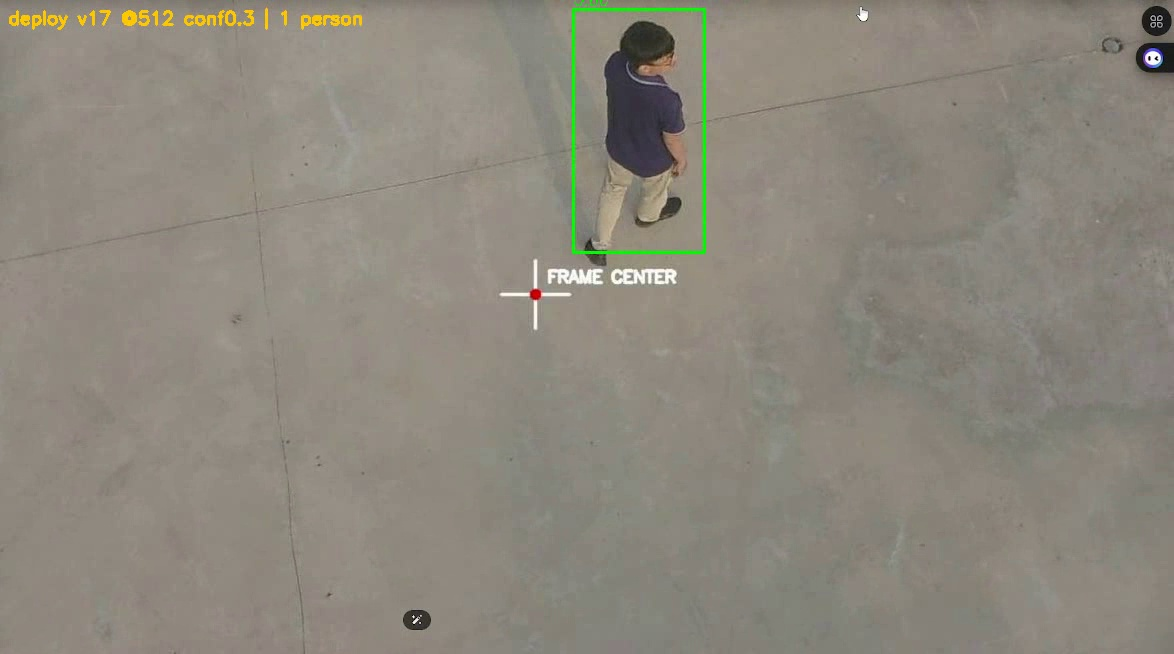
\includegraphics[width=\linewidth]{demo_t15.jpg}\\[-2pt]
{\tiny Khung hình từ chuyến bay thử của đề tài ($\approx$6\,m)}
\end{columns}
\end{frame}

% ------------------------------------------------ 4
\begin{frame}{Khoảng trống nghiên cứu: rung làm bộ phát hiện ``mù''}
\centering
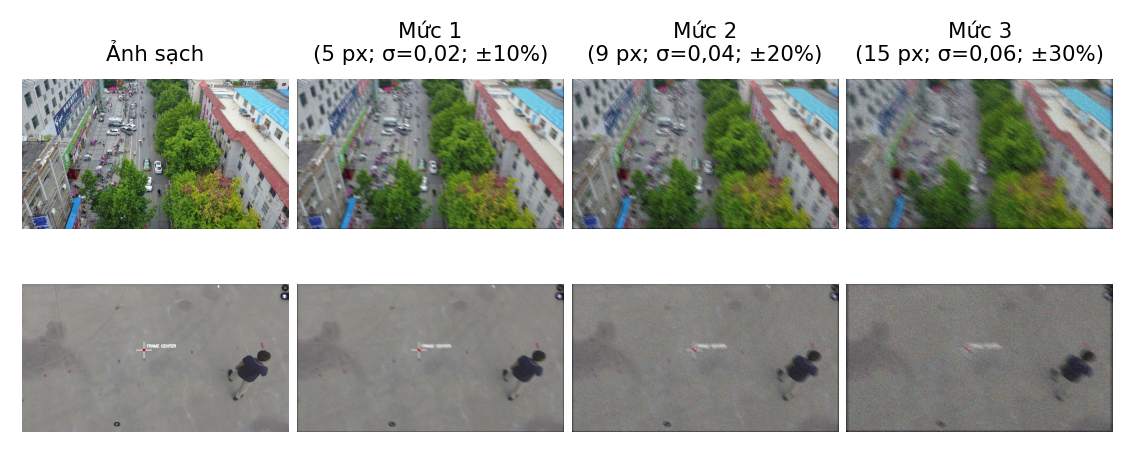
\includegraphics[width=0.7\linewidth]{rung_minh_hoa.png}

\vspace{4pt}
\begin{itemize}
\item Cánh quạt quay $\rightarrow$ camera rung $\rightarrow$ \textbf{nhoè có hướng + nhiễu + dao động sáng}.
\item Các benchmark phát hiện (VisDrone, COCO) chỉ đo trên ảnh sạch.
\item Đo của đề tài: \alert{mọi bộ phát hiện nhỏ gọn mất 74--83\% độ chính xác} khi rung.
\end{itemize}
\end{frame}

% ------------------------------------------------ 5
\begin{frame}{Mục tiêu, phạm vi và phương pháp}
\begin{columns}[T]
\column{0.5\textwidth}
\begin{block}{Mục tiêu (theo thuyết minh)}
\begin{enumerate}
\item Nhận dạng người thời gian thực, độ chính xác \textbf{$\ge$ 70\%}.
\item Thuật toán theo dõi, giữ khoảng cách và hướng bay.
\item Tích hợp camera -- xử lý ảnh -- điều khiển bay ổn định ngoài thực tế.
\end{enumerate}
\end{block}
\column{0.46\textwidth}
\begin{block}{Phương pháp}
\begin{itemize}
\item Học sâu + thị giác máy tính + điều khiển tự động.
\item Thực nghiệm có đối chứng, \textbf{một chương trình đo}, 3 hạt giống.
\item Đo trực tiếp trên phần cứng đích.
\item Kiểm thử phân tầng trước khi bay.
\end{itemize}
\end{block}
\small\textbf{Phạm vi:} một người, không gian thoáng, bay thấp 3--6\,m.
\end{columns}
\end{frame}

% ------------------------------------------------ 6
\begin{frame}{Tổng quan hệ thống}
\centering
\resizebox{!}{0.72\textheight}{% Kiến trúc tổng thể hệ thống UAV bám người
\begin{tikzpicture}[
  font=\footnotesize, >={Stealth[length=2mm]},
  m/.style={draw=black!60, rounded corners=2pt, align=center, minimum height=11mm, text width=2.6cm, inner sep=2pt, fill=white},
  pi/.style={m, fill=xanh!12},
  hw/.style={m, fill=black!6},
  fc/.style={m, fill=cam!14},
  lb/.style={font=\scriptsize, fill=white, inner sep=1pt}
]
% hàng 1: nhận thức
\node[hw] (cam) at (0,0) {Camera C270\\30 khung/giây};
\node[pi] (det) at (3.6,0) {Phát hiện người\\SteadyDet-N INT8};
\node[hw] (npu) at (3.6,1.9) {NPU Hailo-8L};
\node[pi] (trk) at (7.2,0) {Theo vết\\OC-SORT};
\node[pi] (sel) at (10.8,0) {Chọn \& khoá\\mục tiêu};
% hàng 2: điều khiển
\node[pi] (dist) at (10.8,-2.2) {Ước lượng khoảng cách\\pinhole + Kalman};
\node[pi] (servo) at (7.2,-2.2) {Servo thị giác\\3 bộ PID};
\node[pi] (safe) at (3.6,-2.2) {Lớp an toàn\\giới hạn + thang mất MT};
\node[pi] (mav) at (0,-2.2) {MAVLink client\\30\,Hz, chỉ khi GUIDED};
% hàng 3: phần cứng bay + người
\node[fc] (px) at (0,-4.8) {Pixhawk 6C\\ArduPilot};
\node[hw] (mot) at (3.6,-4.8) {Bộ điều tốc\\+ động cơ};
\node[hw, text width=3.0cm] (web) at (7.2,-4.8) {Bảng giám sát web\\(laptop, điện thoại)};
\node[hw] (rc) at (10.8,-4.8) {Tay điều khiển RC\\(người lái)};

\draw[->] (cam) -- (det);
\draw[<->] (det) -- (npu);
\draw[->] (det) -- (trk);
\draw[->] (trk) -- (sel);
\draw[->] (sel) -- (dist);
\draw[->] (dist) -- (servo);
\draw[->] (servo) -- (safe);
\draw[->] (safe) -- (mav);
\draw[<->] (mav) -- node[lb,right]{USB, MAVLink v2} (px);
\draw[->] (px) -- (mot);
\draw[->, dashed] (servo.south) ++(-0.4,0) -- ++(0,-1.45) node[lb,pos=0.5,left]{hình + trạng thái} ;
\draw[<-, dashed] ($(web.north)+(0.4,0)$) -- node[lb,right]{nút đổi mục tiêu} ($(servo.south)+(0.4,0)$);
\draw[->, thick, draw=cam] (rc.south) -- ++(0,-0.55) -| node[lb,pos=0.25,below]{gạt công tắc chế độ bay (luôn ưu tiên)} (px.south);

\begin{scope}[on background layer]
\node[draw=black!45, dashed, rounded corners=4pt, inner sep=7pt, fit=(det)(npu)(trk)(sel)(dist)(servo)(safe)(mav),
      label={[font=\footnotesize\bfseries, anchor=north east]north east:{Raspberry Pi 5 — chương trình \texttt{main.py}}}] {};
\end{scope}
\end{tikzpicture}
}

\vspace{2pt}
{\small Raspberry Pi~5 + NPU Hailo-8L \textbullet\ camera USB \textbullet\ Pixhawk~6C chạy ArduPilot (chế độ GUIDED)}
\end{frame}

% ------------------------------------------------ 7
\begin{frame}{Dữ liệu: hai miền, đánh giá riêng từng miền}
\centering
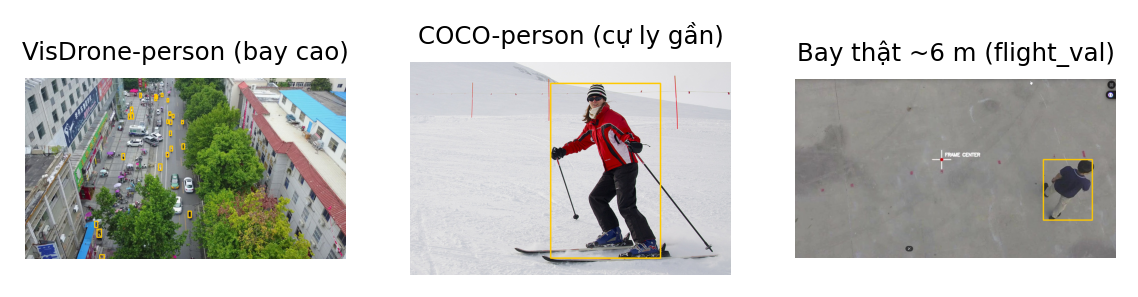
\includegraphics[width=0.88\linewidth]{mau_du_lieu.png}

\vspace{2pt}
\resizebox{0.95\linewidth}{!}{%
\begin{tabular}{@{}lccl@{}}
\toprule
\textbf{Bộ dữ liệu} & \textbf{Ảnh} & \textbf{Hộp} & \textbf{Vai trò}\\\midrule
VisDrone-person (huấn luyện / kiểm định) & 6.471 / 548 & 65.523 / 8.165 & so sánh chuẩn, đánh giá rung\\
COCO-person & 2.654 & 9.783 & bổ sung người cự ly gần\\
Bay thật $\approx$6\,m (flight\_val) & 92 & 92 & \textbf{chỉ đánh giá} miền triển khai\\\bottomrule
\end{tabular}}
\end{frame}

% ------------------------------------------------ 8
\begin{frame}{Giao thức đánh giá VisDrone-Shake}
\begin{columns}[T]
\column{0.5\textwidth}
\[
I_{\text{rung}} = \gamma\,(I * k_{L,\theta}) + n
\]
\small
\begin{tabular}{@{}lccc@{}}
\toprule
\textbf{Mức} & \textbf{Nhoè $L$} & \textbf{Nhiễu $\sigma$} & \textbf{Sáng}\\\midrule
1 (bay treo) & 5\,px & 0,02 & $\pm$10\%\\
2 (bay tiến) & 9\,px & 0,04 & $\pm$20\%\\
3 (rung mạnh) & 15\,px & 0,06 & $\pm$30\%\\\bottomrule
\end{tabular}

\vspace{6pt}
$\mathrm{retain} = 100\cdot\mathrm{mCP}/\mathrm{AP}_{\text{sạch}}$
\column{0.46\textwidth}
\begin{block}{Đo công bằng}
\begin{itemize}\small
\item Nhoè không dịch chuyển vật $\rightarrow$ nhãn giữ nguyên.
\item \textbf{Gieo hạt} + 3 lần lặp: không cố định seed, cùng 1 mô hình cho 17,0 / 17,1 / 17,6\%.
\item \textbf{Một chương trình đo} cho mọi mô hình (khác harness lệch tới 0,01--0,08 AP).
\item Chọn checkpoint theo \textbf{một quy tắc}.
\end{itemize}
\end{block}
\end{columns}
\end{frame}

% ------------------------------------------------ 9
\begin{frame}{Mô hình SteadyDet-N}
\begin{columns}[c]
\column{0.58\textwidth}
\centering\resizebox{!}{0.8\textheight}{% Sơ đồ kiến trúc SteadyDet-N (profile light, ảnh vào 640x640)
\begin{tikzpicture}[
  font=\footnotesize, >={Stealth[length=2mm]},
  blk/.style={draw=black!60, rounded corners=2pt, align=center, minimum height=8.5mm, inner sep=2pt, fill=white},
  bb/.style={blk, fill=black!6, minimum width=3.3cm},
  nk/.style={blk, fill=xanh!10, minimum width=2.2cm},
  hd/.style={blk, fill=cam!12, minimum width=2.4cm},
  p2/.style={dashed, thick},
  lab/.style={font=\scriptsize, text=black!65}
]
% backbone
\node[blk, minimum width=3.3cm, fill=black!2] (in) at (0,0) {Ảnh vào\\$640\times640\times3$};
\node[bb, below=4mm of in] (stem) {EdgeContextStem\\$P_1$: $320^2$, 24 kênh};
\node[bb, below=4mm of stem, p2] (s2) {UIB (1 khối, bước 2)\\$P_2$: $160^2$, 48 kênh};
\node[bb, below=4mm of s2] (s3) {CSP-UIB (2 khối)\\$P_3$: $80^2$, 96 kênh};
\node[bb, below=4mm of s3] (s4) {CSP-UIB (2 khối)\\$P_4$: $40^2$, 144 kênh};
\node[bb, below=4mm of s4] (s5) {CSP-UIB (2 khối)\\$P_5$: $20^2$, 192 kênh};
\node[bb, below=4mm of s5, fill=xanh!22] (att) {Window self-attention\\(chỉ ở $P_5$)};
\foreach \a/\b in {in/stem,stem/s2,s2/s3,s3/s4,s4/s5,s5/att} \draw[->] (\a) -- (\b);

% neck (top-down)
\node[nk, right=2.3cm of att] (n5) {Conv $1\times1$\\48 kênh};
\node[nk, above=9.5mm of n5] (n4) {UIB\\48 kênh};
\node[nk, above=9.5mm of n4] (n3) {UIB\\48 kênh};
\node[nk, above=9.5mm of n3, p2] (n2) {UIB\\24 kênh};
\draw[->] (att) -- node[lab,above]{chiếu $1\times1$} (n5);
\draw[->] (s4.east) -- ++(0.9,0) |- (n4.west);
\draw[->] (s3.east) -- ++(0.7,0) |- (n3.west);
\draw[->] (s2.east) -- ++(0.5,0) |- (n2.west);
\draw[->, xanh, thick] (n5) -- node[lab,right]{$\uparrow2$, cộng} (n4);
\draw[->, xanh, thick] (n4) -- node[lab,right]{$\uparrow2$, cộng} (n3);
\draw[->, xanh, thick] (n3) -- node[lab,right]{$1\times1$, $\uparrow2$, cộng} (n2);

% heads
\node[hd, right=1.9cm of n2, p2] (h2) {LiteHead\\ra $160^2\times5$};
\node[hd, right=1.9cm of n3] (h3) {LiteHead\\ra $80^2\times5$};
\node[hd, right=1.9cm of n4] (h4) {LiteHead\\ra $40^2\times5$};
\node[hd, right=1.9cm of n5] (h5) {LiteHead\\ra $20^2\times5$};
\foreach \a/\b in {n2/h2,n3/h3,n4/h4,n5/h5} \draw[->] (\a) -- (\b);

\node[lab, above=1mm of s2.north east, anchor=south west, xshift=-4mm] {};
\node[font=\footnotesize\bfseries] at (0,1.0) {Backbone};
\node[font=\footnotesize\bfseries] at (n2 |- 0,1.0) {FPN neck (từ trên xuống)};
\node[font=\footnotesize\bfseries] at (h2 |- 0,1.0) {Head};
\node[draw=black!40, rounded corners=2pt, fill=black!3, align=left, font=\scriptsize, text width=3.9cm, below=6mm of h5] (lh)
 {\textbf{LiteHead:} DW $3\times3$ + PW $1\times1$ dùng chung $\rightarrow$ 1 kênh điểm người + 4 kênh hộp (hồi quy trực tiếp, không DFL).\\[2pt]
  Nét đứt: nhánh $P_2$ bước 4 được làm mỏng (1 khối, nửa số kênh neck, head depthwise separable).};
\end{tikzpicture}
}
\column{0.4\textwidth}
\begin{itemize}\footnotesize
\item \so{1,17 triệu tham số, 4,6 GFLOPs}.
\item Giữ mức $P_2$ (bước 4) cho \textbf{người nhỏ}.
\item Nhánh $P_2$ \textbf{mỏng}: 1 khối, nửa số kênh.
\item Tính toán dồn về $P_3$--$P_5$ (bản đồ nhỏ).
\item Head depthwise separable.
\item Rẻ hơn bản trước (12,9 GFLOPs) \textbf{2,8 lần}.
\item Hàm mất mát: QFL + NWD/CIoU theo diện tích.
\end{itemize}
\end{columns}
\end{frame}

% ------------------------------------------------ 10
\begin{frame}{Huấn luyện nhận biết rung}
\centering
\resizebox{0.85\linewidth}{!}{% Sơ đồ huấn luyện nhận biết rung (trên) và biến thể ràng buộc nhất quán (dưới)
\begin{tikzpicture}[
  font=\footnotesize, >={Stealth[length=2mm]},
  box/.style={draw=black!60, rounded corners=2pt, align=center, minimum height=9mm, inner sep=3pt, fill=white},
  op/.style={box, fill=cam!14},
  net/.style={box, fill=xanh!14, minimum width=2.1cm},
  loss/.style={box, fill=black!7},
  dec/.style={diamond, draw=black!60, aspect=2.2, inner sep=1pt, align=center, fill=white, font=\scriptsize}
]
\node[font=\footnotesize\bfseries, anchor=west] at (-0.4,1.1) {(a) Huấn luyện nhận biết rung (phương pháp đề xuất)};
\node[box] (x) at (0,0) {Lô ảnh $x$\\+ nhãn $y$};
\node[dec, right=6mm of x] (d) {xác suất\\$p=0{,}5$};
\node[op, right=7mm of d] (T) {Toán tử rung $\mathcal{T}$\\nhoè $L,\theta$ + nhiễu $\sigma$ + sáng $b$};
\node[net, right=7mm of T] (f) {Mạng\\$f_\theta$};
\node[loss, right=7mm of f] (L) {$\mathcal{L}_{\det}\big(f_\theta(\hat{x}), y\big)$\\nhãn giữ nguyên};
\draw[->] (x) -- (d);
\draw[->] (d) -- node[above,font=\scriptsize]{có} (T);
\draw[->] (T) -- node[above,font=\scriptsize]{$\hat x$} (f);
\draw[->] (d.south) -- ++(0,-0.55) -| node[pos=0.25,below,font=\scriptsize]{không: $\hat x = x$} (f.south);
\draw[->] (f) -- (L);

\begin{scope}[yshift=-3.75cm]
\node[font=\footnotesize\bfseries, anchor=west] at (-0.4,1.5) {(b) Biến thể ràng buộc nhất quán (đối chứng, cho kết quả kém hơn)};
\node[box] (x2) at (0,0) {Lô ảnh $x$\\+ nhãn $y$};
\node[net] (fc) at (4.2,0.75) {$f_\theta(x)$ nhánh sạch};
\node[op] (T2) at (2.0,-0.75) {$\mathcal{T}$};
\node[net] (fv) at (4.2,-0.75) {$f_\theta(\tilde x)$ nhánh rung};
\node[loss, anchor=west] (Ld) at (7.4,0.75) {$\mathcal{L}_{\det}(f_\theta(x), y)$};
\node[loss, anchor=west] (sg) at (7.4,-0.75) {$\lambda\,\mathcal{L}_{\text{cons}}\big(f_\theta(\tilde x),\ \mathrm{sg}[f_\theta(x)]\big)$};
\draw[->] (x2.east) -- ++(0.35,0) |- (fc.west);
\draw[->] (x2.east) -- ++(0.35,0) |- (T2.west);
\draw[->] (T2) -- node[above,font=\scriptsize]{$\tilde x$} (fv);
\draw[->] (fc) -- (Ld);
\draw[->] (fv) -- (sg);
\draw[->, dashed] (fc.east) ++(0.2,0) -- node[left,font=\scriptsize, pos=0.5]{dừng gradient} ($(sg.north west)+(0.4,0)$);
\end{scope}
\end{tikzpicture}
}

\vspace{4pt}
\begin{columns}[T]
\column{0.48\textwidth}\small
\textbf{(a) Đề xuất:} thay 50\% lô bằng ảnh rung, tính hàm mất mát phát hiện bình thường. \alert{Không đổi mô hình khi suy luận.}
\column{0.48\textwidth}\small
\textbf{(b) Đối chứng:} ràng buộc nhất quán (2 lượt truyền xuôi, tốn 1,8$\times$ thời gian) --- kết quả \textbf{kém hơn}.
\end{columns}
\end{frame}

% ------------------------------------------------ 11
\begin{frame}{Kết quả chính và các đối chứng (VisDrone-person)}
\centering
\resizebox{\linewidth}{!}{%
\begin{tabular}{@{}lcccc@{}}
\toprule
\textbf{SteadyDet-N} & \textbf{AP sạch} & \textbf{AP mức 2} & \textbf{retain (\%)} & \textbf{Kết luận}\\\midrule
Gốc & 0,1892 & 0,0123 & 16,8 $\pm$ 0,7 & ``mù'' khi bay tiến\\
+ 120 epoch không rung & 0,1823 & 0,0125 & 16,9 $\pm$ 0,7 & huấn luyện thêm vô ích\\
+ ràng buộc nhất quán & 0,1746 & 0,0392 & 30,0 $\pm$ 0,6 & kém hơn, tốn 1,8$\times$\\
\textbf{+ huấn luyện nhận biết rung} & 0,1708 & \so{0,0518} & \so{36,2 $\pm$ 0,7} & \textbf{tốt nhất}\\\midrule
SteadyDet-W: gốc $\rightarrow$ rung & 0,2349 $\rightarrow$ 0,2219 & 0,0258 $\rightarrow$ 0,0839 & 22,2 $\rightarrow$ 39,4 & tái lập được\\
YOLO11-n: gốc $\rightarrow$ rung & 0,2588 $\rightarrow$ 0,2579 & 0,0248 $\rightarrow$ 0,0227 & 21,9 $\rightarrow$ 21,5 & không tác dụng\\\bottomrule
\end{tabular}}

\vspace{8pt}
\begin{block}{}
retain \textbf{16,8\% $\rightarrow$ 36,2\%}; AP ở mức rung bay tiến \textbf{tăng 4,2 lần}; AP sạch chỉ giảm 9,7\%.
\end{block}
\end{frame}

% ------------------------------------------------ 12
\begin{frame}{So sánh với 5 mô hình nhẹ: thứ hạng đảo ngược khi rung}
\begin{columns}[c]
\column{0.5\textwidth}
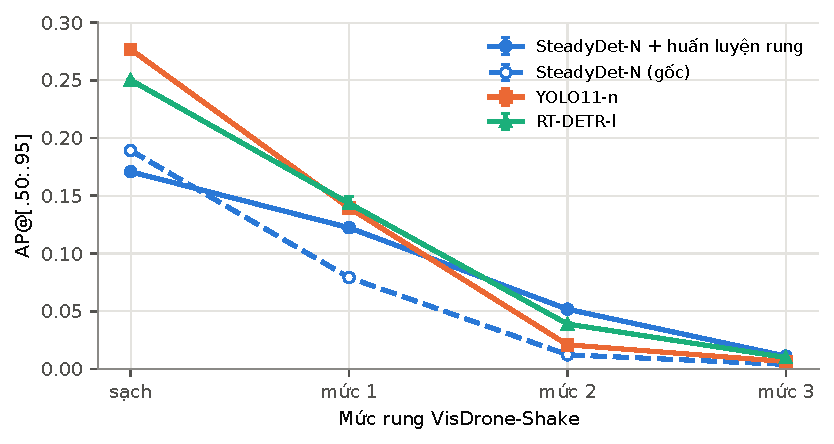
\includegraphics[width=\linewidth]{duong_cong_rung.pdf}
\column{0.48\textwidth}\scriptsize
\begin{tabular}{@{}lccc@{}}
\toprule
\textbf{Mô hình} & \textbf{GFLOPs} & \textbf{AP sạch} & \textbf{mCP}\\\midrule
RT-DETR-l & 108,0 & 0,2502 & 0,0641\\
YOLO11-n & 6,4 & \textbf{0,2768} & 0,0557\\
YOLOv10-n & 8,4 & 0,2730 & 0,0538\\
YOLOv8-n & 8,2 & 0,2684 & 0,0522\\
YOLO26-n & 5,8 & 0,2675 & 0,0507\\
SteadyDet-W + rung & 12,9 & 0,2219 & \so{0,0874}\\
\textbf{SteadyDet-N + rung} & \textbf{4,6} & 0,1708 & \so{0,0617}\\\bottomrule
\end{tabular}

\vspace{4pt}
\small
\begin{itemize}
\item Ảnh sạch: SteadyDet-N \textbf{thua}.
\item Khi rung: \textbf{vượt cả 4 YOLO nano} với 45\% tham số; ở mức 2 vượt RT-DETR-l (lớn 28$\times$).
\end{itemize}
\end{columns}
\end{frame}

% ------------------------------------------------ 13
\begin{frame}{Kiểm chứng trên dữ liệu bay thật (92 khung)}
\begin{columns}[c]
\column{0.55\textwidth}
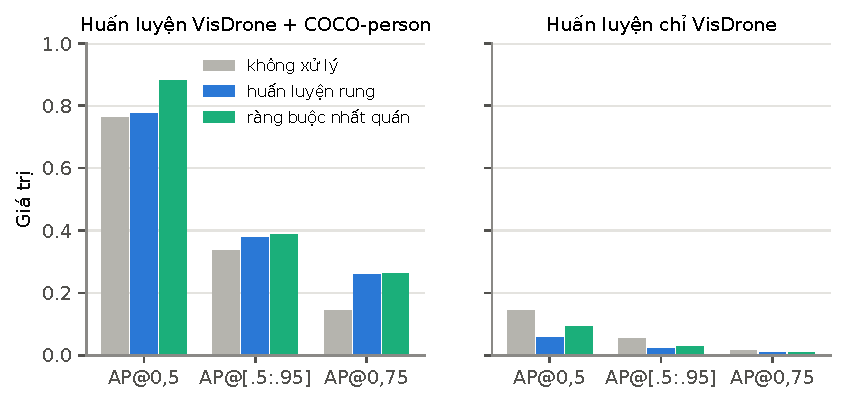
\includegraphics[width=\linewidth]{bay_that.pdf}
\column{0.43\textwidth}
\begin{itemize}\small
\item Có COCO-person: AP@0,5 \textbf{gấp 5,3 lần} chỉ VisDrone $\rightarrow$ \alert{chọn dữ liệu theo miền triển khai}.
\item Xử lý rung: AP@0,75 \textbf{+78\% / +81\%} (hộp khít hơn), khoảng tin cậy bootstrap 95\% không chứa 0.
\item Hạn chế: 1 người, 1 cảnh, 1 độ cao.
\end{itemize}
\end{columns}
\end{frame}

% ------------------------------------------------ 14
\begin{frame}{Triển khai trên Raspberry Pi 5 + Hailo-8L}
\begin{columns}[c]
\column{0.55\textwidth}
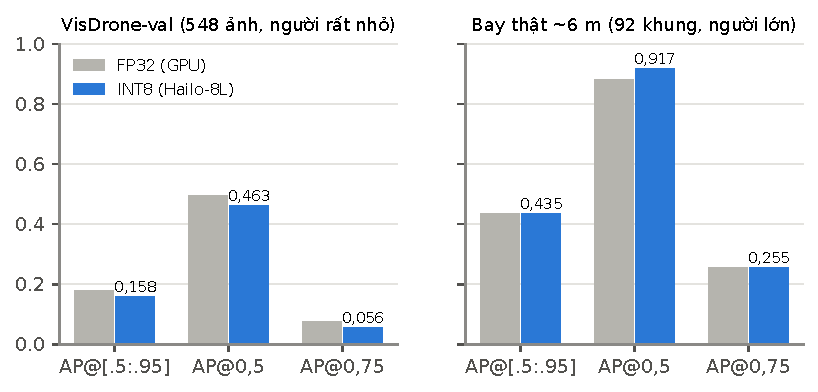
\includegraphics[width=\linewidth]{int8.pdf}
\column{0.43\textwidth}\small
\begin{itemize}
\item INT8: \so{AP@0,5 = 0,917} trên bay thật; F1 = 0,880 (ngưỡng 0,25).
\item Tổn thất INT8 phụ thuộc kích thước vật: $-6{,}5\%$ với người rất nhỏ, $\approx 0$ ở 3--6\,m.
\item NPU: \textbf{112,55 FPS} @320, \textbf{63,66 FPS} @640 (lô 1).
\item \textbf{Nhanh hơn YOLO26-n 1,70 lần} (4 so với 6 context).
\end{itemize}
\end{columns}
\end{frame}

% ------------------------------------------------ 15
\begin{frame}{Độ trễ đầu-cuối: hệ thống bị giới hạn bởi camera}
\centering
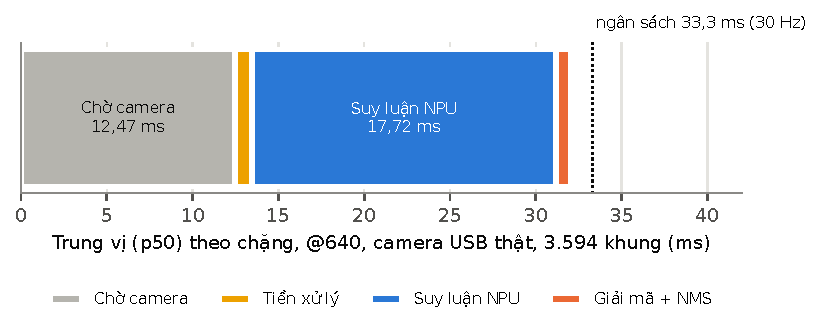
\includegraphics[width=0.72\linewidth]{do_tre.pdf}

\begin{columns}[T]
\column{0.5\textwidth}\small
\begin{itemize}
\item Đầu-cuối \so{30,0 FPS}, p50 32,04\,ms, p99 36,15\,ms.
\item Tính toán chỉ 19,55\,ms / 33,3\,ms (59\%).
\item 48,5\,°C, không giảm xung sau 2 phút.
\end{itemize}
\column{0.46\textwidth}\small
\begin{itemize}
\item Sửa 2 lỗi camera: bộ đệm = 1 rớt nửa khung; tự phơi sáng hạ FPS.
\item \textbf{11,1 $\rightarrow$ 30,0 FPS} không đổi mô hình.
\end{itemize}
\end{columns}
\end{frame}

% ------------------------------------------------ 16
\begin{frame}{Hệ thống điều khiển bám người}
\begin{columns}[c]
\column{0.36\textwidth}
\centering\resizebox{!}{0.78\textheight}{% Lưu đồ một vòng lặp điều khiển 30 Hz
\begin{tikzpicture}[
  font=\footnotesize, >={Stealth[length=2mm]},
  st/.style={draw=black!60, rounded corners=2pt, align=center, minimum height=8mm, text width=5.2cm, inner sep=2pt, fill=white},
  sm/.style={st, text width=3.6cm},
  io/.style={st, fill=xanh!12},
  dc/.style={diamond, draw=black!60, aspect=2.8, align=center, inner sep=0pt, fill=cam!10, font=\scriptsize, text width=2.4cm},
  tm/.style={st, rounded corners=9pt, fill=black!8}
]
\node[tm] (s) at (0,0) {Bắt đầu vòng lặp (chu kỳ 33,3\,ms)};
\node[io] (a) at (0,-1.1) {1. Lấy khung mới nhất từ camera};
\node[st] (b) at (0,-2.2) {2. Phát hiện người trên NPU (ngưỡng 0,25; NMS)};
\node[st] (c) at (0,-3.3) {3. Cập nhật bộ theo vết OC-SORT};
\node[st] (d) at (0,-4.4) {4. Chọn/khoá mục tiêu (xử lý nút đổi mục tiêu)};
\node[io] (e) at (0,-5.5) {5. Đọc trạng thái máy bay qua MAVLink};
\node[dc] (f) at (0,-6.9) {Có mục tiêu?};
\node[sm] (g) at (-3.4,-8.4) {6. Khoảng cách pinhole + Kalman $\rightarrow$ 3 PID $\rightarrow$ giới hạn an toàn};
\node[sm] (h) at (3.4,-8.4) {Đặt lại các bộ PID};
\node[st] (i) at (0,-9.9) {7. Cập nhật thang mất mục tiêu\\8. Kiểm tra sức khoẻ hệ thống};
\node[dc] (j) at (0,-11.5) {Đang ở GUIDED?};
\node[sm, fill=xanh!12] (k) at (-3.4,-13.0) {9. Gửi vận tốc: FOLLOW / COAST ($\times0{,}5$) / HOVER (0)};
\node[sm] (l) at (3.4,-13.0) {Không gửi lệnh (người lái đang giữ quyền)};
\node[st] (m) at (0,-14.5) {10. Ghi log CSV, cập nhật bảng giám sát};
\foreach \x/\y in {s/a,a/b,b/c,c/d,d/e,e/f,i/j} \draw[->] (\x) -- (\y);
\draw[->] (f.west) -| node[pos=0.25,above,font=\scriptsize]{có} (g.north);
\draw[->] (f.east) -| node[pos=0.25,above,font=\scriptsize]{không} (h.north);
\draw[->] (g.south) |- (i.west);
\draw[->] (h.south) |- (i.east);
\draw[->] (j.west) -| node[pos=0.25,above,font=\scriptsize]{có} (k.north);
\draw[->] (j.east) -| node[pos=0.25,above,font=\scriptsize]{không} (l.north);
\draw[->] (k.south) |- (m.west);
\draw[->] (l.south) |- (m.east);
\draw[->] (m.south) -- ++(0,-0.4) -- ++(6.0,0) |- (s.east);
\end{tikzpicture}
}
\column{0.62\textwidth}\small
\begin{itemize}
\item \textbf{OC-SORT}: giữ vết 1,5\,s, xác nhận sau 3 lần phát hiện.
\item \textbf{Khoá mục tiêu} hộp lớn nhất; tìm lại người cũ 5\,s theo vị trí + cỡ hộp; nút \emph{Đổi mục tiêu}.
\item \textbf{Khoảng cách} $Z = f_y H_r / h$ + Kalman; giữ 5\,m.
\item \textbf{3 PID}: tiến lùi, quay hướng ($e=(u-W/2)/f_x$), độ cao.
\end{itemize}
\scriptsize
\begin{tabular}{@{}lcccc@{}}
\toprule
\textbf{Kênh} & $K_p$ & $K_i$ & $K_d$ & \textbf{Giới hạn}\\\midrule
Tiến lùi & 0,5 & 0,05 & 0,1 & $\pm$3\,m/s\\
Quay hướng & 2,0 & 0 & 0,3 & $\pm$1,5\,rad/s\\
Độ cao & 0,8 & 0,1 & 0,2 & $\pm$2\,m/s\\\bottomrule
\end{tabular}
\end{columns}
\end{frame}

% ------------------------------------------------ 17
\begin{frame}{Nhịp lệnh 30 Hz và lớp an toàn}
\begin{columns}[c]
\column{0.5\textwidth}
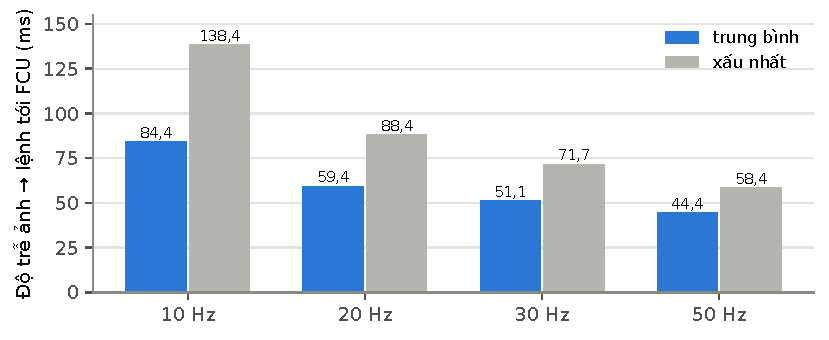
\includegraphics[width=\linewidth]{nhip_lenh.pdf}
{\scriptsize Khứ hồi lệnh p50 4,75\,ms / p99 7,73\,ms, 0\% mất gói tới 50\,Hz. 30\,Hz = đúng nhịp bộ phát hiện.}
\column{0.48\textwidth}
\resizebox{\linewidth}{!}{% Máy trạng thái thang mất mục tiêu
\begin{tikzpicture}[
  font=\footnotesize, >={Stealth[length=2mm]},
  s/.style={circle, draw=black!60, align=center, minimum size=19mm, inner sep=1pt, fill=white},
]
\node[s, fill=xanh!15] (F) {FOLLOW\\\scriptsize bám theo};
\node[s, fill=cam!12, right=3.2cm of F] (C) {COAST\\\scriptsize vận tốc $\times0{,}5$};
\node[s, fill=black!8, right=3.2cm of C] (H) {HOVER\\\scriptsize vận tốc 0};
\draw[->] (F) to[bend left=18] node[above,font=\scriptsize,align=center]{mất mục tiêu} (C);
\draw[->] (C) to[bend left=18] node[below,font=\scriptsize]{thấy lại} (F);
\draw[->] (C) -- node[above,font=\scriptsize,align=center]{mất $\ge$ 3\,s} (H);
\draw[->] (H) to[bend left=35] node[below,font=\scriptsize]{thấy lại mục tiêu} (F);
\draw[->] (H) edge[loop right] node[right,font=\scriptsize,align=left]{đứng yên đến khi\\người lái gạt\\công tắc chế độ} (H);
\end{tikzpicture}
}
\begin{itemize}\small
\item Giới hạn vận tốc, khoảng cách 3--15\,m, độ cao 2--25\,m.
\item Kiểm tra GPS, pin 4S, heartbeat.
\item \textbf{Chỉ gửi lệnh khi GUIDED}; \texttt{GUID\_TIMEOUT} 1\,s.
\end{itemize}
\end{columns}
\end{frame}

% ------------------------------------------------ 18
\begin{frame}{Vòng bám người trên video bay thử}
\centering
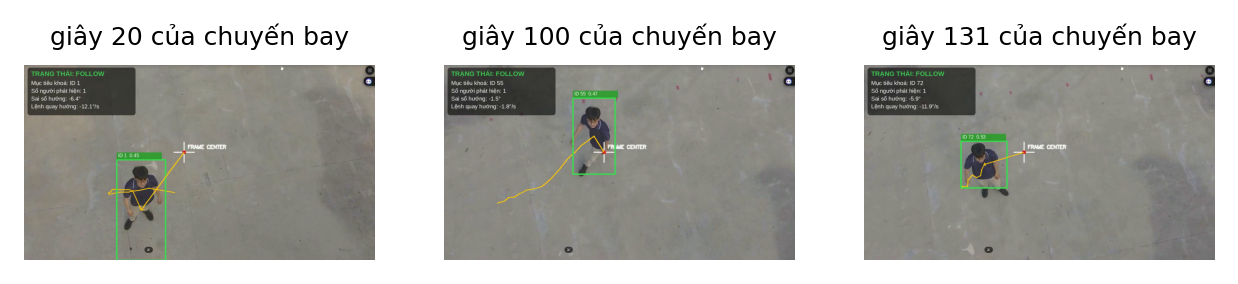
\includegraphics[width=0.95\linewidth]{vongbam_khung.png}

\vspace{4pt}
\begin{columns}[T]
\column{0.48\textwidth}\small
\begin{itemize}
\item Chuyến bay 21/07/2026 ($\approx$6\,m), 3.961 khung.
\item SteadyDet-N $\rightarrow$ OC-SORT $\rightarrow$ khoá mục tiêu $\rightarrow$ PID quay hướng $\rightarrow$ FOLLOW / COAST / HOVER.
\end{itemize}
\column{0.48\textwidth}\small
\begin{itemize}
\item Giữ mục tiêu \so{83,5\%} thời gian; đoạn liên tục dài nhất 25,4\,s.
\item Sai số hướng khi bám: trung vị \so{5,5$^\circ$}.
\item Mất phát hiện ngắn: COAST theo dự đoán rồi bám lại.
\end{itemize}
\end{columns}
\end{frame}

% ------------------------------------------------ 19
\begin{frame}{Video bay thử}
\begin{columns}[c]
\column{0.62\textwidth}
\href{run:../video/video_bay_thu.mp4}{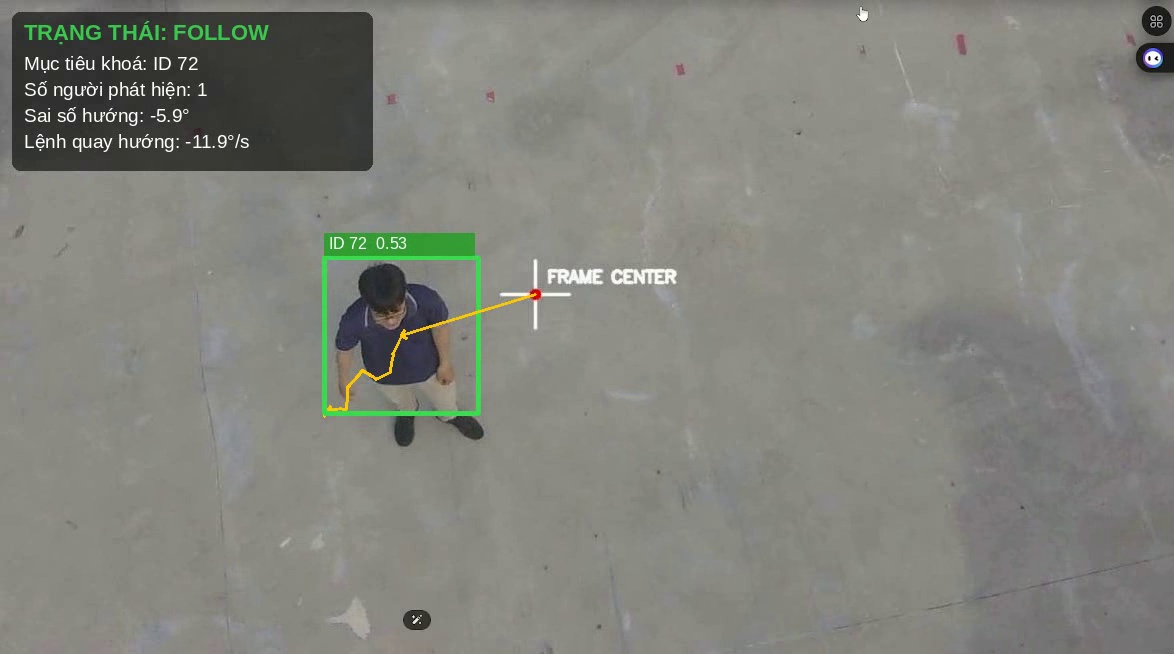
\includegraphics[width=\linewidth]{vongbam_3.jpg}}
\column{0.36\textwidth}\small
\begin{itemize}
\item Chuyến bay 21/07/2026, độ cao $\approx$6\,m.
\item Phần 1: SteadyDet-N phát hiện người trên từng khung hình.
\item Phần 2: vòng bám người khoá mục tiêu và tính lệnh điều khiển.
\end{itemize}
\vspace{6pt}
\beamerbutton{\href{run:../video/video_bay_thu.mp4}{Bấm để phát video (4 phút 43 giây)}}

{\scriptsize Tệp: \texttt{video/video\_bay\_thu.mp4}}
\end{columns}
\end{frame}

% ------------------------------------------------ 20
\begin{frame}{Đánh giá mức độ đạt mục tiêu}
\small
\begin{tabularx}{\linewidth}{@{}>{\raggedright\arraybackslash}p{4.2cm}>{\raggedright\arraybackslash}p{2.8cm}>{\raggedright\arraybackslash}X@{}}
\toprule
\textbf{Mục tiêu / sản phẩm} & \textbf{Yêu cầu} & \textbf{Kết quả}\\\midrule
Nhận dạng người thời gian thực & $\ge$ 70\% & \so{AP@0,5 = 91,7\%}, F1 0,880, 30 FPS --- \textbf{vượt}\\
Theo dõi, giữ khoảng cách, hướng & ổn định & OC-SORT, khoá/tìm lại mục tiêu, pinhole + Kalman, 3 PID, 30\,Hz --- \textbf{đạt}\\
Tích hợp hệ thống & ổn định thực tế & 7 tầng kiểm thử, bay thử; vòng bám giữ mục tiêu 83,5\% thời gian --- \textbf{đạt}\\
Chương trình máy tính & 01 & Mã nguồn đầy đủ + kiểm thử --- \textbf{đạt}\\
Báo cáo tổng kết & 01 & Báo cáo, tóm tắt, poster, video bay thử --- \textbf{đạt}\\\bottomrule
\end{tabularx}
\end{frame}

% ------------------------------------------------ 21
\begin{frame}{Kết luận và hướng phát triển}
\begin{columns}[T]
\column{0.5\textwidth}
\begin{block}{Kết luận}
\footnotesize
\begin{itemize}
\item UAV tích hợp nhận dạng và bám người, xử lý hoàn toàn trên máy bay.
\item Rung làm mọi bộ phát hiện nhỏ gọn mất 74--83\% độ chính xác.
\item Huấn luyện nhận biết rung tăng gấp đôi độ bền, \textbf{0 chi phí suy luận}.
\item Mô hình nhỏ nhất vượt 4 YOLO nano khi rung; nhanh hơn YOLO26-n 1,70 lần trên NPU.
\end{itemize}
\end{block}
\column{0.46\textwidth}
\begin{block}{Hướng phát triển}
\footnotesize
\begin{itemize}
\item Hiệu chuẩn mô hình rung bằng nhật ký IMU.
\item Mở rộng dữ liệu bay thật nhiều độ cao, nhiều người.
\item Đưa mô hình nhận biết rung lên NPU.
\item Mở rộng bay bám nhiều kịch bản; nhận dạng lại theo ngoại hình.
\end{itemize}
\end{block}
\end{columns}
\end{frame}

% ------------------------------------------------ 22
{\setbeamertemplate{footline}{}
\begin{frame}[plain]
\begin{tikzpicture}[remember picture,overlay]
\fill[dam] (current page.north west) rectangle (current page.south east);
\node[text=white,font=\Huge\bfseries] at ($(current page.center)+(0,0.6)$) {XIN CẢM ƠN};
\node[text=white,align=center,font=\normalsize] at ($(current page.center)+(0,-0.8)$) {Kính mong nhận được góp ý của Quý Thầy Cô trong Hội đồng};
\node[text=white,align=center,font=\small] at ($(current page.south)+(0,1.2)$) {\chunhiem{} \textbullet\ \emailchunhiem};
\end{tikzpicture}
\end{frame}}
\end{document}
